\section{Discussion}
\subsection{Classification}
The classification results are fairly accurate, looking at the accuracy assessment metrics. Especially the vegetation class is classified very well, having 98\% of the points classified as vegetation also being vegetation. The irrelevant class, which is mostly composed of buildings, railway power lines and ditches, is less accurate with 72\% of the points correctly classified. 

When analysing these statistics it is important to take the removal of the majority of the points in consideration. A major part of the irrelevant points were removed before the classification. The irrelevant points left share many similarities with vegetation points and are consequently much harder to classify correctly.

Improving the classification could be tried in a number of ways. We identified four areas which can be changed for a better result.

Firstly, the result of the feature importance assessment could be used to make a selection of the more important features and only use those in the classification. This could be a way to improve the result, as irrelevant features can decrease the performance of a classifier, and decrease the computation time, as less features lead to simpler trees~\citep{rogers2006identifying}.

Secondly, other techniques to tackle the unbalanced data problem could also present different results. Instead of adjusting the sampling technique within the random forest algorithm it is also possible to oversample the minority class or undersample the majority class before using a machine learning algorithm. This can be done randomly, but also in smart ways, using algorithms such as SMOTE (Synthetic Minority Over-sampling Technique) or ADASYN (Adaptive Synthetic Sampling) for oversampling~\citep{chawla2002smote, he2008adasyn}, and Condensed Nearest Neighbor (CNN) or Tomek Links for undersampling~\citep{hart1968condensed, tomek1976two}.

Thirdly, the classification result might also be improved by using a different machine learning algorithm. Algorithms like SVM~\citep{mallet2008analysis, zhang2013svm, weinmann2015semantic} and Adaboost~\citep{lodha2007aerial, weinmann2015semantic} have been proven to be effective classifiers and could potentially offer a better classification result.

Lastly, selecting another neighbourhood could provide better results as well. Spherical or cylindrical neighbourhoods could be used instead, or the \(k\)-nearest neighbourhood could be improved by finding optimal values for \(k\). This can for example be done by minimizing the eigenenthropy (equation~\ref{eq:eigenentropy}) for a range of \(k\)~\citep{weinmann2014semantic}. While this results in a slightly improved classification, the computational effort required is high.

For our purpose however a complete accurate result is not necessary, as we want to delineate the linear vegetation elements for which we need most of the vegetation points correctly classified, but not all. The classification result show most of the incorrectly classified points are dispersed and surrounded by correctly classified points. These scattered points do not impact the subsequent delineation of linear objects. If desired these points could be cleaned up by looking at a neighbourhood around each point and changing its classification if a very large majority of those points are of a different class.

\subsection{Delineating Linear Objects}
The comparison of the manual with automated delineation shows that linear objects were generally accurately extracted, evidenced by the accuracy scores. When interpreting these scores it is important to keep in mind the degree of interpretation which is required when creating the manual classification. The rules for when a vegetation object is linear are ambiguous and thus open for varying interpretations. 

The automated delineation shows a few additions and omissions with our interpretation. The linear objects at 1 and 2 (figure~\ref{fig:linear}) are the biggest omission in the automated delineation compared to the manual one. Closer inspection of the rectangular objects in this area reveal that this area is segmented as a series of rectangle-like objects instead of a single more elongated element. This is the result of the distribution of the trees in rows of two to three across a dike (see figure~\ref{fig:omission}). These objects are by themselves not linear and do not get merged because they are not aligned. Omissions at 3, 4 and 5 are the result of the downsampling of the point cloud before the automated delineation. The tree lines at 3 are composed of very young and thin trees and consequently have too few points for the creation of proper rectangular objects. Position 4 might suffer from this as well, but also contains physical gaps between the trees. The low vegetation at 5 has similar problems. There are also places where the automated method delineates linear objects which are not part of the manual delineation. Positions 6, 7 and 8 are examples of this. The trees at 6 are part of a larger vegetation patch which includes both low vegetation and trees. A human is prone to see this as a single patch and thus not a linear element, while a machine does not make this interpretation. The forest patches at 7 and 8 get classified as linear elements because they are on the border of the research area and are cut off. Without this cut off the objects would not be seen as a linear element.

\begin{figure}
	\centering
	\fbox{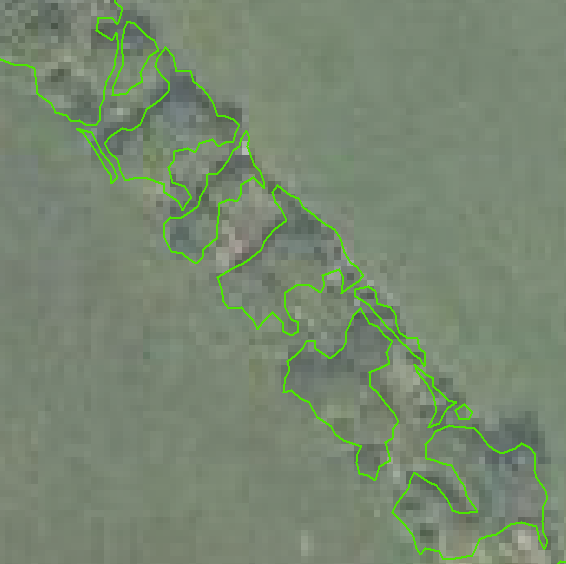
\includegraphics[scale=0.6]{./img/omission1}}
	\caption{Detail of the omission at 1.}
	\label{fig:omission}
\end{figure}

The results show a few main limitations of the method. Firstly, the computation time is fairly high. Therefore a compromise has to be made between precision and time. The resulting downsampling of the points can cause small objects to be ignored. Secondly, the objects are not always merged correctly. The merging is done based on the orientation and alignment of the two objects, which works well in most cases. The orientation of an object however is only meaningful when it is somewhat elongated, which is not the case for single trees for example. A row of separated single trees will consequently not be merged and seen as a linear element. The alignment of objects can also prevent some objects, which could be seen as one object, to be merged. This can be seen at position 1, as the objects are in a row of unaligned pairs of trees. Lastly, when vegetation is mixed the method might delineate linear objects, while this might not be desirable. If a mixed vegetation should be seen as one object the delineation of linear objects could be done before the classification into low vegetation and trees.

Despite these limitations the method is successful in delineating the large majority of the linear elements present in the research area, which contains linear and non-linear vegetation patches of many different shapes.

\subsection{Future outlook}
Even though the research area was chosen to cover many different shapes of linear and non-linear vegetation patches the method should be validated using more and different areas, both within the AHN3 dataset as datasets of different countries. This should be done without retraining the classifier. If this fails a more general applicable classifier needs to be created.

The automated nature of the method means it can be upscaled to large areas. The linear vegetation elements can be delineated for the whole AHN3 dataset for example, eventually spanning the entire country of the Netherlands. This would require quite some computational power, but high performance computing paradigms like cloud computing or supercomputing can provide the power needed. The method is written using FOSS and should be able to run in such an environment. The dataset could be split up into smaller parts and run in parallel.

National LiDAR datasets are becoming increasingly available for European countries besides the Netherlands, such as in Denmark, England, Finland, Slovenia, Spain, Sweden and Switzerland. With minor alterations the method should be able to work with these datasets as well, making it possible to cover a large part of Europe.

The resulting database of tree lines and hedges throughout the Netherlands or Europe could be used as an extra indicator for ecosystem health and biodiversity in agricultural landscapes. This could provide an improvement in ecosystem and biodiversity assessments, such as the MAES (Mapping and Assessment of Ecosystems and their Services) project~\citep{maes2013mapping}, the SEBI (Streamlining European Biodiversity Indicators) project~\citep{biala2012streamlining}, and the high nature value 
farmland assessment~\citep{paracchini2008high} on a European scale and assessments of Planbureau voor de Leefomgeving (PBL) on a national level~\citep{bouwma2014biodiversiteit}.

Additionally the results could be used for further ecological and physical geographical research. Tree lines and hedges play an important role, for example, in the distribution of species and in the microclimate of fields. They have an influence on varying fluxes, such as wind and water flows, soil erosion and animal movement~\citep{forman1984hedgerows}. It could consequently be used as a parameter in a species distribution model, or to analyse the relation between linear elements and certain animal species, or to estimate the stability of soil.

The method can also be used for other purposes. Other landscape elements, like roads and ditches, can also be segmented using this technique. These elements also influence the ecosystem as barriers and corridors. The automated delineation of roads is also subject of research outside of ecology~\citep{quackenbush2004review}.



